\chapter{A Walk through Las Rozas}
\vspace{0.6cm}
\begin{center}
\nopagebreak
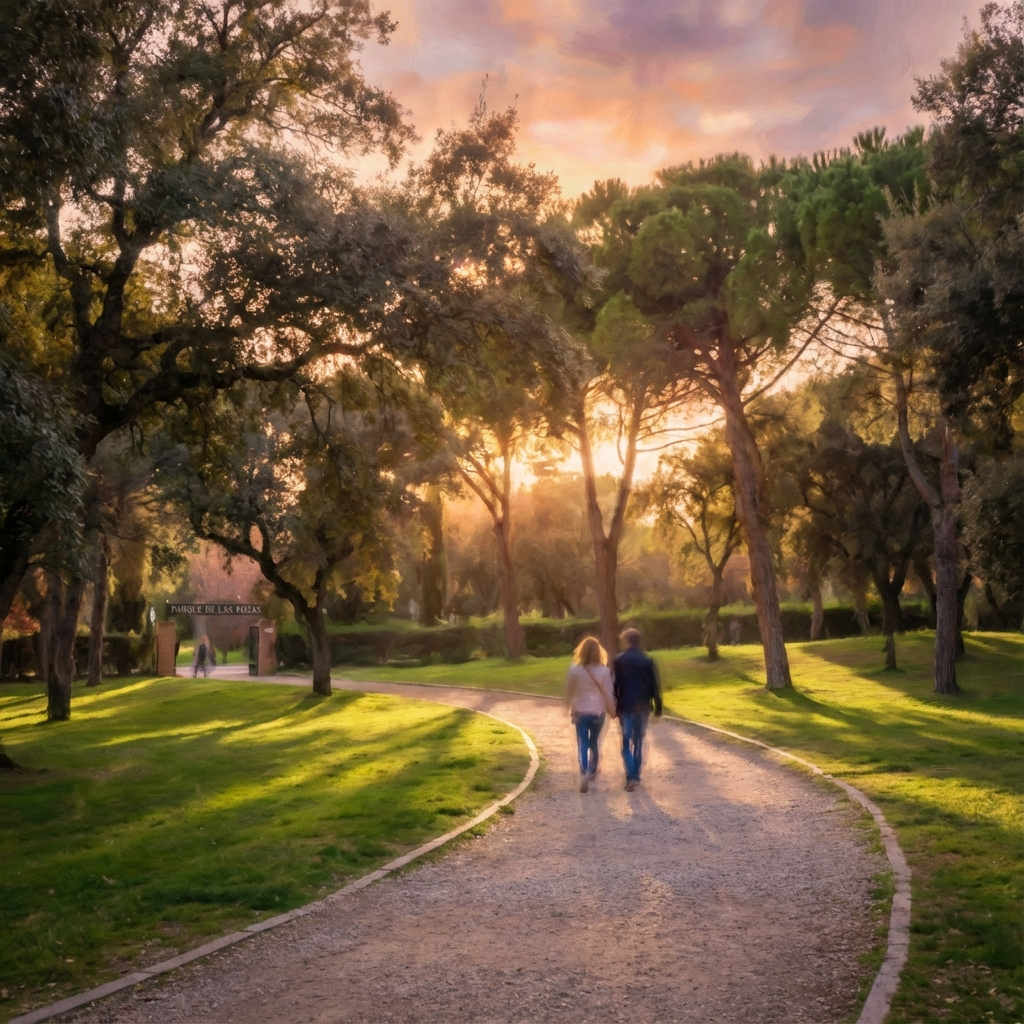
\includegraphics[width=0.75\textwidth,cfbox=gray!60 0.6pt 4pt]{las_rozas_park.png}\\
\vspace{4pt}
{\small\itshape The silence of the park: tuning the inner temple.}
\end{center}

\vspace{0.6cm}
The next day, we decided to get away from the center a bit. We went to Las Rozas. Jesus wanted to see how people lived in the outskirts, in those developments where everything seems orderly, but where chaos sometimes hides behind armored doors.


We were walking through Paris Park. He stopped to smell the flowers, to touch the bark of the trees.
—Do you see this? —he told me, pointing to an oak—. He doesn't worry about whether it will rain tomorrow or if it will be sunny. He simply is. He is in his center. He vibrates at the frequency of life.


—It's easy for a tree —I replied—. It doesn't have a mortgage.


Jesus laughed out loud. A clean, infectious laugh.
—The mortgage... the great modern monster. Look, Francisco, the problem isn't the bank debt. The problem is the debt you think you have with the future. You live paying in advance with your anxiety for a time that doesn't yet exist.


We sat on the grass. A dog came running and licked his hand. He petted it tenderly.
—``Give us this day our daily bread'' —he whispered—. People think I only talk about food. I'm talking about the energy needed for the \textit{now}. When you worry about next month, you are spending today's energy on an imaginary problem. You lower your vibration. You weaken yourself.


—And how do you raise the vibration? —I asked, feeling that I was beginning to understand.


—By being grateful —he said, looking at the artificial lake—. Gratitude is the elevator of the soul. If you are grateful for this sun, this air, this moment... you go up. If you complain about what you lack... you go down. It's basic spiritual physics.


In Las Rozas, between villas and high-end cars, I learned that true wealth was not in what we possessed, but in the ability to enjoy what was already there, free, for everyone.